\section{Geodésicas}

\begin{frame}
	\frametitle{Geodésicas}
	\begin{definition}
		Sea $M$ una variedad suave equipada con una conexión afín $\nabla$. Diremos que una curva $\gamma: [a,b] \to M$ es una \textbf{curva geodésica} si:
		\[
			\nabla_{\gamma'(t)} \gamma'(t) = 0
		\]
	\end{definition}
\end{frame}

\begin{frame}
	\frametitle{Existencia y unicidad de geodésicas}
	\begin{theorem}
		Sea $M$ una variedad suave equipada con una conexión afín. Para cada punto $p \in M$, cada vector tangente $v \in T_{p}M$ y cada real $t_0$ existe un intervalo abierto $I \subset \mathbb{R} $ que contiene a $t_0$ y una geodésica $\gamma(t) : I \to M $ que satisface $\gamma(t_0) = p$ y $\gamma'(t_0) = v$. \pause Cualesquiera dos geodésicas que satisfagan las mismas condiciones coincidirán en la intersección de sus dominios.
	\end{theorem}

\end{frame}

\begin{frame}
	\frametitle{Existencia y unicidad de geodésicas}
	\begin{proof}
		\begin{enumerate}
			\item Como se mencionó anteriormente, dada una carta $(U,\phi)$ se puede expresar a la conexión en términos de las coordenadas locales como:
			      \[
				      \nabla_{\gamma'(t)}\gamma'(t) = \sum_{k=1}^{n} \left(
				      \frac{d\gamma'_k(t)}{dt} + \sum_{i=1}^{n}\sum_{j=1}^{n} \frac{d\gamma_{i}(t)}{dt} \Gamma_{ij}^{k}\gamma_{j}'(t)
				      \right) \partial_{k}			      \] \pause
			\item Por definición de geodésica, $\nabla_{\gamma'(t)}\gamma'(t) = 0$, esto ocurre si y solo si:
			      \[
				      \gamma''_{k}(t) + \sum_{i=1}^{n}\sum_{j=1}^{n} \Gamma_{ij}^{k}\gamma_{i}'(t) \gamma_{j}'(t) = 0
			      \]
		\end{enumerate}
	\end{proof}
\end{frame}

\begin{frame}
	\frametitle{Existencia y unicidad de geodésicas}
	\begin{proof}
		\begin{enumerate}
			\setcounter{enumi}{2}
		\item Esta ecuación, a la cual se le llama la \textbf{ecuación geodésica}, puede ser reducida realizando la sustitución $\gamma''(t) = x'(t)$, de modo que obtenemos:
			      \[
				      x_{k}'(t) + \sum_{i=1}^{n} \sum_{j=1}^{n} \Gamma_{ij}^{k} x_{i}(t) x_{j}(t) = 0.
			      \] \pause
			\item El teorema de existencia y unicidad de las ecuaciones diferenciales ordinarias garantiza que este sistema tendrá solución y dicha solución será única.
		\end{enumerate}
	\end{proof}
\end{frame}

\begin{frame}
	\frametitle{Geodésicas en $\mathbb{H}^2$}
	\begin{definition}[Espacio hiperbólico de dimensión $2$]
		Consideremos al subconjunto de $\mathbb{R}^{2}$:
		\[
			\mathbb{H}^{2} = \{(x,y) : x \in \mathbb{R}, y > 0\},
		\]\pause
		este subconjunto es un abierto en $\mathbb{R}^{2}$, por lo cual es una variedad topológica, este subconjunto puede ser cubierto por una única carta, por lo cual está determina una estructura suave. \pause Hacemos de $\mathbb{H}^{2}$ una variedad Riemanniana dotándolo de la métrica cuyos coeficientes son:
		\[
			g_{ij} = \frac{R \delta_{ij}}{y^{2}}, \quad R \in \mathbb{R}
		\]\pause
		a esta variedad Riemanniana se le conoce como \textbf{espacio hiperbólico de dimensión 2} o \textbf{modelo de Poincaré del semiplano superior}.
	\end{definition}
\end{frame}

\begin{frame}
	\frametitle{Geodésicas en $\mathbb{H}^2$}
	Para calcular las geodésicas en el $\mathbb{H}^{2}$ comenzamos calculando los símbolos de Christoffel. \pause
	\[
		\Gamma_{ij}^{m} = \frac{1}{2} \sum_{k=1}^{2}(\partial_{i} g_{jk} + \partial_{j} g_{ki} - \partial_{k}g_{ij})g^{km}
	\]\pause

	\begin{columns}[t]
		\column{.1\textwidth}
		\begin{align*}
			\Gamma_{11}^{1} & = 0           \\[12pt]
			\Gamma_{11}^{2} & = \frac{1}{y}
		\end{align*}
		\column{.1\textwidth}
		\begin{align*}
			\Gamma_{12}^{1} & = -\frac{1}{y} \\[12pt]
			\Gamma_{21}^{1} & = -\frac{1}{y}
		\end{align*}
		\column{.1\textwidth}
		\begin{align*}
			\Gamma_{12}^{2} & = 0 \\[24pt]
			\Gamma_{21}^{2} & = 0
		\end{align*}
		\column{.1\textwidth}
		\begin{align*}
			\Gamma_{22}^{1} & = 0            \\[12pt]
			\Gamma_{22}^{2} & = -\frac{1}{y}
		\end{align*}
	\end{columns}
\end{frame}

\begin{frame}
	\frametitle{Geodésicas en $\mathbb{H}^2$}
	Si $\gamma$ es una curva podemos suponer que está parametrizada como $\gamma(t) = (x(t),y(t))$, \pause si $\gamma(t)$ es una curva geodésica al sustituir estas parametrizaciones y los símbolos de Christoffel en la ecuación geodésica obtendremos el sistema de ecuaciones diferenciales:
	\[
		\begin{cases}
			x'' - \frac{2}{y} x'y'                         & = 0 \\[12pt]
			y'' + \frac{1}{y} (x')^2 - \frac{1}{y}(y')^{2} & = 0
		\end{cases}
	\] \pause

	Las soluciones de este sistema de ecuaciones son las siguientes:
	\vspace{12pt}
	\begin{columns}
		\column{0.4\textwidth}
		\centering
		Si $x'(t) = 0$, \\[12pt]
		$y = y_{0}e^{kt}$
		\column{0.4\textwidth} \pause
		\centering
		Si $x'(t) \neq 0$, \\[12pt]
		$(x - C)^{2} + y^{2} = \frac{k_0}{K_{1}^{2}}$
	\end{columns}
\end{frame}

\begin{frame}
	\frametitle{Geodésicas en $\mathbb{H}^2$}
	\begin{figure}[h]
		\centering
		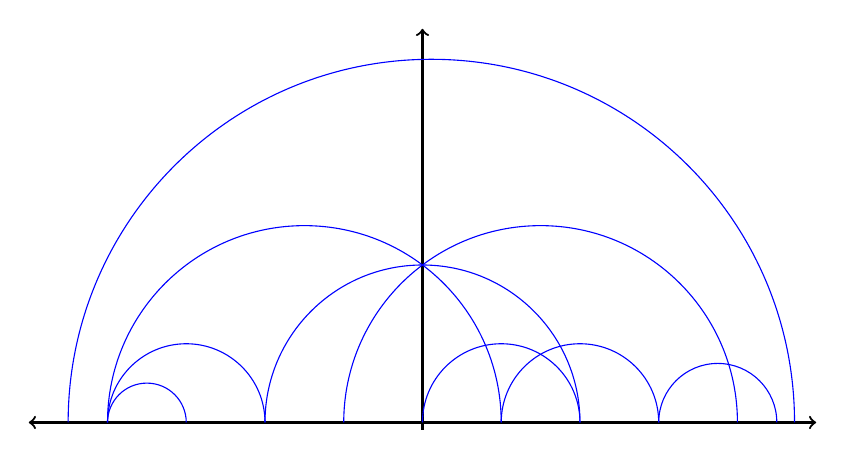
\begin{tikzpicture}
  \draw[color=black,thick,<->] (-5,0) -- (5,0);
  \draw[color=black,thick,<-] (0,5) -- (0,-0.1);

  \draw[blue] (2,0) arc (0:180:1);
  \draw[blue] (2,0) arc (0:180:2);
  \draw[blue] (3,0) arc (0:180:1);
  \draw[blue] (3,0) arc (180:0:0.75);
  \draw[blue] (-1,0) arc (180:0:2.5);
  \draw[blue] (-4,0) arc (180:0:2.5);
  \draw[blue] (-4,0) arc (180:0:0.5);
  \draw[blue] (-4,0) arc (180:0:1);
  \draw[blue] (-4.5,0) arc (180:0:4.6125);
\end{tikzpicture}

		\caption{Representación de algunas geodésicas en $\mathbb{H}^{2}$}
	\end{figure}
\end{frame}
